\subsection{Audio, PWM}\label{sec:audioPWM}
Um ein Audiosignal abspielen zu können, werden zwei PWM-Signale benötigt wie in Abbildung . Das einte Signal ist die invertierte Variante des anderen Signals. 
Das PWM-Signal wird mit dem NRF52 generiert. Für den NRF52 stellt NORDIC SEMICONDUCTOR die PWM HAL and driver Bibliothek zu Verführung, die es ermöglicht ein PWM zu erzeugen. Der NRF52 bietet vier PWM Instanzen mit je vier Kanälen. In der Tabelle sind die Funktionen aufgelistet die aus dieser Bibliothek verwendet werden. Auf diese zwei Funktionen wird im folgenden Abschnitt eingegangen. 

\textbf{Bild von zwei PWM Ausgängen.}

\begin{table}[]
	\centering
	\begin{tabular}{|l|l|l|}
		\hline
		%\rowcolor[HTML]{C0C0C0} 
		\textbf{Beschreibung} & \textbf{Funktion}                & \textbf{Argumente}                                                                                                                                                                                                            \\ \hline
		PWM initialisiern     & nrf\_drv\_pwm\_init              & \begin{tabular}[c]{@{}l@{}}nrf\_drv\_pwm\_t const *const p\_instance\\ nrf\_drv\_pwm\_config\_tconst *p\_config\\ nrf\_drv\_pwm\_handler\_thandler\end{tabular}                                                               \\ \hline
		Audio abspielen         & nrf\_drv\_pwm\_complex\_playback & \begin{tabular}[c]{@{}l@{}}nrf\_drv\_pwm\_t const *const p\_instance\\ nrf\_pwm\_sequence\_t const *p\_sequence\_0\\ nrf\_pwm\_sequence\_tconst *p\_sequence\_1\\ uint16\_t  playback\_count \\ uint32\_t  flags\end{tabular} \\ \hline
	\end{tabular}
	\label{my-label}
	\caption{Funktionen der PWM HAL and driver Bibliothek}
\end{table}

\subsubsection{Konzept}\label{sec:Konzept}
In der Abbildung \ref{fig:pwm_ablauf} ist der Ablauf des PWM-Unterprogramm aufgezeigt. Als erstes muss die Initialisierung statt finden. Nach der Initialisierung können die beiden Sequenzen 0 und 1 generiert werden. In diesen Sequenzen sind die wav file Daten abgelegt. Mit diesen Sequenzen wird ein PWM Signal erzeugt. Dies geschieht mit der Funktion complex\_playback.

\begin{figure}[H]
	\begin{center}
		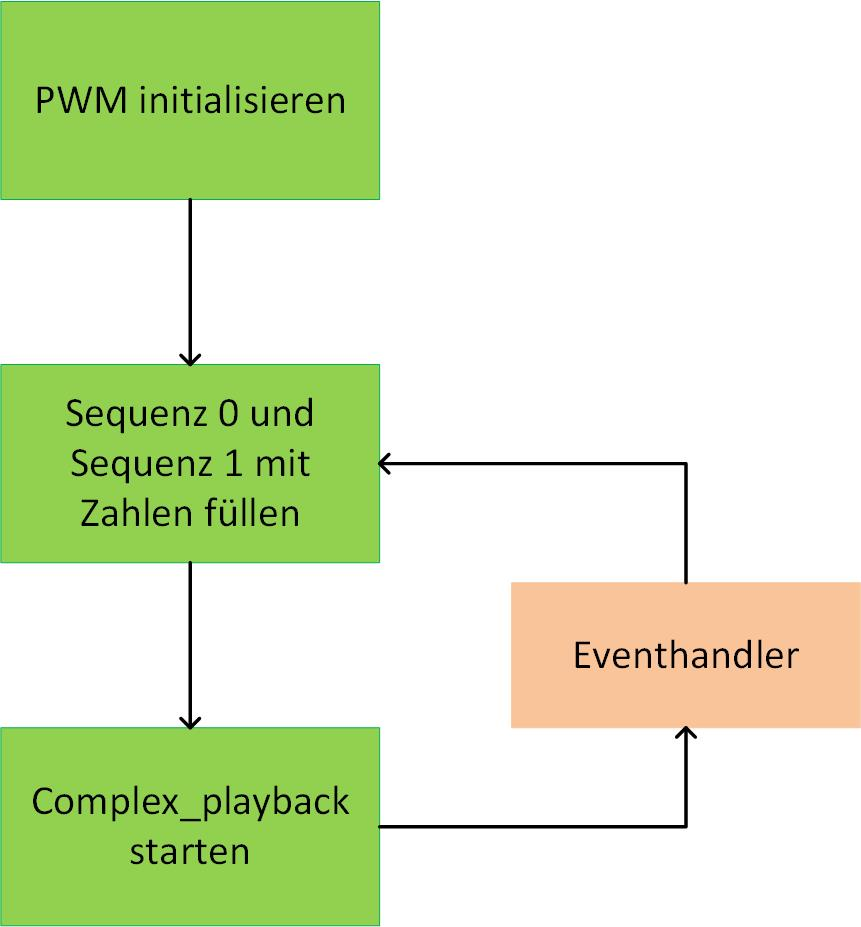
\includegraphics[width=80mm]{data/pwm_ablauf.jpg}
		\caption[Ablauf PWM]{Ablauf PWM} %picture caption
		\label{fig:pwm_ablauf}
	\end{center}
\end{figure}

\subsubsection*{PWM Initialisieren}\label{sec:PWM initialisieren}
Definieren der Abtastfrequenz
-Welche PWM Instanz\\
-Config\\
	*ouputPins\\
	*clock\\
	*zählermodus\\
	*top value\\
	*Kanal modus\\
	*modus\\
-event handler

\subsubsection*{Sequenzen befüllen}\label{sec:Sequenzen befüllen}
Daten in sequenzen füllen, seqeuenz 1 muss noch ein Datenwert dazugerechnet werden. verweisen auf die SD Kart lesefunktion.

\subsubsection*{Complex playback}\label{sec:Complex playback}
Vorteil zu simple playback ist das zwei sequenzen mitgegeben werden können. Wenn die Sequenz 0 fertig abgespielt wurde, startet automatisch die zweite Sequenz und der eventhandler wird ausgelöst. In dieser Zeit kann die erste Sequenz wieder neu befüllt werden. Die Befüllung der Sequenzen wird mit dem eventhandler dieser Funktion gesteuert. 
